\newpage

% Chapter 2
\begingroup%
\makeatletter%
\let\clearpage\relax% Stop LaTeX from going to a new page; and
\vspace*{\fill}%
\vspace*{\dimexpr-50\p@-\baselineskip}% Remove the initial (default) 50pt gap (plus 1 line)
\chapterfont{\centering}
\chapter{Literature Review}
\vspace*{\fill}%
\endgroup

\newpage
\label{Chapter2}
\lhead{Chapter 2. \emph{Literature Review}} % Write in your own chapter title to set the page header

\justifying
In this section, we are going to discuss virtual reality, applications that did work on E-Commerce applications with VR, AR, and a comparison of different web applications.
\section{Details of Existing Work}
\justifying
We are living in an era where technology is evolving at a rapid pace and so is the traditional way of work or business. For example, On-site classes are slowly switching to online classes, cash-on-hand payment is slowly switching to online payment, manual Registration, reservations, booking, etc are also being switched to online, so technology has greatly affected our traditional tasks. Now, it is evolving to virtual reality-based works to facilitate the users even more than before. The term “metaverse” has been on-trend in recent times. It is a concept in which people can collaborate and live their life virtually in the virtual world using VR headsets. So far it is in the initial stages but many single-purpose apps have already implemented this feature. In our relevant cases, many e-commerce and clothing stores have started working on this virtual try-before-you-buy feature. Usually, the try-before-you-buy technique is used by customers when shopping physically but many stores such as \cite{IkeaWala} Ikea have started Kitchen virtual reality in which a person can walk freely and interact with the virtual kitchen using a VR headset. Virtual 3-D Kitchen items can be tested in this environment. They also \cite{ekIkeaWala} has launched a new augmented reality application that allows users to test their products in real-time. So far it can only be used with Apple technology(ARKit). The app automatically scales products based on the given environment with 98 percent accuracy.
The E-Commerce websites like Amazon, Alibaba, AliExpress, Walmart, etc., and outerwear websites like Zeitgeist, breakout have traditional approaches where customers go on the websites and then see different product items and add to card method.
In today’s modern world, the need for technology with an E-commerce system has become a basic need. People need a more personalized and immersive shopping 
experience which makes the way for the meta verse concept. With the expansion of the industrial metaverse, Virtual shopping still needs learning, priorities,
 and insights for experience delivery \cite{"FutureofE-Commerce"}
\section{What is Virtual Reality?} 
\justifying
Virtual Reality is the future and it's a 3D complete environment in which everything provides a real-time feeling. Virtual reality is a buzzword today and it is popular nowadays in the future students can take lessons and classes in a virtual environment and companies like Amazon is also working on e-commerce virtual reality-based application. People can just wear a VR headset and in their homes, they can go to virtual e-commerce stores, and explore mental health treatment. There are lots of applications of virtual reality like VR in fashion design, mental health treatment, education, sports, military, medical training, etc.

\section{Difference between Virtual Reality and \\ Augmented Reality}

\justifying
No external AR headset is required for experiencing augmented reality while a VR headset is required for experiencing a virtual environment. In virtual reality, everything is virtual like objects in a virtual environment while Augmented reality augments the real-world scene. Snapchat uses augmented reality when we open a Snapchat camera then Snapchat provides different filters in which we can different objects The filters in which Snapchat lens scans our face and applies different cartoon shapes or filters or face changers etc. all possible because of augmented reality.

\section{Current State of Art}
        \begin{longtable}{| L{1cm} | L{2cm} | L{3cm} | L{2cm} | L{4cm} |}
            \hline
            \rowcolor{Gainsboro!60}
            \makecell{ } & \makecell{Name}  & \makecell{Category} & \makecell{Status} & \makecell{Function}
            \endhead
            1&	Yihaodian	& AR Store & Onsite&	AR stores created on open spaces that give customers the experience of real-world stores in smartphones .\cite{Yihaodian} \\
           \hline
2	& IKEA	& Catalog Application	& Online &	Customers can use AR technology in their smartphones to preview how furniture will look in that surrounding by augmenting furniture objects in real-world \cite{IKEA}\\
           \hline
3	& Lacoste	& LCST Augmented Reality Retail Campaign &	Online	&Customers can try different shoes . \cite{Lacoste}\\
           \hline
4	& Audi	& VR-Based Application &	On-Site	& Passengers traveling with a driver and feeling bored can experience amusing 3D environments configured with real-world vehicle speed, and bumps on the road in the real world by wearing VR headsets provided by AUDI .\cite{Audi} \\
           \hline
                5	& Converse	& Shoe Sampler & 	Online	& Customers can try shoes by using AR-based applications.\cite{Converse} \\
           \hline
6 &	Topshop	& AR Mirror &	In-Store &	Customers can try-on outfits in-store by using AR change room. \cite{Topshop}\\
           \hline
7 & Sephora &	AR-based application &	Online	& Customers can get virtual makeup and try different shades by using Sephora virtual assist in their mobile phones\cite{Sephora} \\
           \hline
8 &	L’Oréal	& AR-based application	& Online &	Customers can try out all L’Oréal products by using virtual makeovers and can try different beauty trends on their mobile phones, and tablets.\cite{Loreal}\\
           \hline
           9	& Burberry &	Virtual Store	& Online	& Customers will experience the virtual store by navigating through the 3D store environment and would be selecting products by selecting digital icons in the environment. \cite{Burberry} \\
           \hline
10	& Mister Spex	& Virtual Mirror &	Online	& Customers can try different frames of glasses virtually using AR-based applications and can find his/her favorite model.\cite{MisterSpex} \\
           \hline
         11 &	Timber Land	& AR Magic mirror	& In-Store &	Customers can tryout different outfits by standing in front of their avatar in mirror screen .\cite{TIMBERLAND}\\
           \hline
 12 &	Uniqlo &	AR Mirror 	& In-Store &	Customers can try different colors of a single cloth product by just wearing that single product in front of an AR-based mirror called “magical mirror”.\cite{UNIQLO}    \\
           \hline
13	& Gapinc &	AR-based application	& Online &	Customers can virtually try on clothes using an AR app called Dressing Room by GAP\cite{Gapinc} \\
           \hline
           \caption{
           Comparison of existing AR and VR-based applications.}
        \end{longtable}

This table discussed the existing AR/VR-based applications and their functionalities. These applications were developed by some famous companies like Audi, Converse, Sephora, and many others listed in the table. These companies brought new innovations to their respective field by using AR/VR technology. Such that Audi developed an application to kill the boring time of their users by providing them with a VR headset with amusing VR environments. The fusion of these amusing and enjoyable VR environments with car speed, acceleration and road bumps, and cuts made Audi’s customers attracted to this innovation.      
%\end{landscape}

\subsection{IKEA}
\justifying
IKEA made an application that used augmented reality by which customers can place the IKEA furniture at any place and can see how it will look at that place. For example, if you want to see how the table will look in your room then using the IKEA application you just have to open the camera same as Snapchat, and then you can see the place the object anywhere. So customers can place different IKEA furniture in any place like in their home. They just have to open the IKEA application and select a product and using the back camera of their mobile phone they can see how the furniture i.e table will look in their room. \cite{IKEA}
\subsection{Yihaodian}
Yihaodian is launching a virtual online grocery store based on augmented reality where customers. Yihaodian is one of the largest grocery online stores that work on buying groceries with AR experience to improve customer satisfaction and customer experience of buying products online.
\cite{Yihaodian}
\subsection{Lacoste}
\justifying
Customers can try different shoes with AR experience.
Using our extensive AR experience we developed a LCST app allowing consumers to “Bring the Colour” to their city by scanning store window displays, in-store signage, and promotional postcards to reveal exclusive 3D video animation content to consumers across 6 global territories. The AR activity helped successfully launch the new Lacoste streetwear brand by showcasing LCST as the bold, edgy choice in the urban sportswear market.\cite{Lacoste}
\subsection{Audi}
	Audi has developed a project named “holoride” in which they have tried to improve passenger rides. They have stated the problem situation when someone travels with a driver in an Audi car. At that time driver enjoys the ride but the passenger considers that time as wasted time. So Audi has tried to kill that boring time with a unique AR/VR experience. So they have used “Extended Reality(XR)” to build some beautiful and enjoyable VR experiences that passengers can experience while having a ride just by wearing a VR headset. 
The cool thing in this “holoride” is the relationship between the real world and the virtual environment. In the virtual world, passengers will be riding on some 3d objects like a cart, or an animal-like dinosaur based on the VR environment the passenger would be in. So there would be a fusion of real-world data with a VR environment such that the speed of the ride in the environment would be the same as the speed of the car in the real world. Similarly, with each bend on the road, with each application of the brake, the virtual reality experience would be shaped just like the real world. 
They have just replaced the boring passenger experience of the real world with a fascinating, colorful, and amusing virtual reality experience. \cite{Audi}

\subsection{Converse}
 The converse is a shoemaker company that has created an AR app to ease users with a fitting facility without leaving home.
Converse not only solved customers’ pain but also reduced its sales funnel. They have created an AR app in which users can see if the shoes fit him/her by using AR technology. The user just has to open the AR camera and select his/her favorite shoes and just point the camera toward his feet to see shoes fit or not.
There was a gap in online shoe shopping which was size fitting. But this technology eliminated this gap in online shopping.
 \cite{Converse}
 
\subsection{Topshop}
TOPSHOP a renowned fashion brand launched an augmented reality shopping tool, TOPSHOP Kinect, that helps their customers to try on their selected collections in an augmented dressing room. They worked with the Russian agency AR Door and launched the augmented reality dressing room in Moscow. They use Microsoft's Xbox Kinect software to create virtual mirrors.
Users simply must pose with their arms headed upward and allow the Kinect to take the picture. Then viewers can move their hands and check different styles that are inside the application. Kinect’s built-in camera scans the body and places the selected dress concerning the user's every movement. Its changing room is the first of its kind to hit major retail stores.\cite{Topshop}
\subsection{Sephora}
\justifying
Sephora introduced a mirror-like application in which a person can test the makeup toolkit accurately with the actual motive to make the person through AR and not with the conventional technique. It checks for the precise location of a user’s facial features, making it to be the world’s first photo-realistic 3D mirror. Try-on technology and Digital dress-up are its two major functionalities. \cite{Sephora}
\subsection{L'Oreal}L'Oréal's Modiface brings an AI-powered Virtual Makeup setup. Customers can apply makeup and try different shades to use virtual artists on their mobile phones. ModiFace, a leader in augmented reality and artificial intelligence in the beauty industry provided its AI-powered technology for cosmetic try-on virtually.
\cite{Sephora}
\subsection{Burberry}
Burberry, a fashion house, collaborated with ELLE Digital Japan in its latest move to create an interactive virtual copy of the Ginza store. They upgraded themselves through creative innovations and explored the relationship between physical and digital experiences for creating new concepts.
Customers can now roam around the virtual store and purchase items from Burberry’s inventory.
The store is built over three floors: the ground floor contains signature bags. The first floor contains womenswear from key outerwear. The top floor includes menswear and outerwear. Burberry and ELLE Digital Japan and in collaboration with actress Elaiza Ikeda created styling films that can be accessed through the virtual store.\cite{Burberry}
\subsection{Mister Spex}
It provides an amazing experience in that you can see how different glass frames will look on you in the virtual mirror and this is all you can do in your home on the Mister Spex website.
\subsection{Timber Land}
This clothing brand took the relationship with the audience and the experience to a new level. The mobile app was used initially for fitting in AR mode. Now people don't even have to go to the store. They just have to reach an 80-inch monitor and a full-length character appears on the screen. This approach resulted in a positive and incredible review by people and they started to use this AR fitting service in queues. Sharing of results of virtual fitting via Facebook and email is also possible.\cite{TIMBERLAND}
\subsection{Uniqio}
UNIQLO started initiatives to decrease environmental waste and support hawker culture, where people from over Singapore gather at hawker centers to dine. They created exhibition displays and augmented reality murals at UNIQLO stores. 
They provided an interactive experience by pointing to their mobile phones. Customers can also unlock face filters on Instagram after scanning the AR mural, granting them access to take selfies.
\\
The company aims to incorporate its efforts into eradicating environmental waste combined with AR technology. The company is looking to further its efforts into environmental waste, combined with newly released AR technology.\cite{UNIQLO}
\subsection{Gapinc}
Gapinc.Gap introduced Virtual Dressing and unveiled a new pilot app called the Dressing Room by Gap. The app was created to help customers virtually “try on" clothing through a smartphone, Augmented Reality experience. This is how it works – shoppers choose a Gap style that they might be interested in purchasing. Next, they select one of five body types featured in the app so they can “try on" the piece of clothing from anywhere on a Google Tango-enabled device, and if they love it, they can buy it online.
The fashion industry has not traditionally been geared toward helping people understand how clothes will fit. But Gapinc is determined and passionate about winning customer trust by consistently presenting and delivering products that make them look and feel great.\cite{Gapinic}

\section{Research Gap}
The previous E-Commerce work never used any virtual stores or virtual environments in which different products were placed and customers can visit the virtual store in their homes just by wearing VR headsets. In short, there is no current such a website that is having a virtual environment where customers can just come into the virtual store while wearing a VR headset and when a customer clicks on the dress he/she can see the avatars wearing the outfits like a jacket and the customer can also see the detailed information like different sizes of outfits (For example jackets). As to buying outerwear customers have two options first one is to order online and the second one is to go to the mall or store to buy outerwear. Another option is the augmented reality the customer just opens the camera and can try on different outfits because of the augmented reality. 
Another, gap we found is that there are 2D images of outfits and the models wearing those outfits are also in 2D images instead of the 3D model. Like a 3D image in which a person wearing outfits and customers can see back and forth how actually outfit will look like when any person will wear it.
            \begin{center}
             \captionof{table}{Research work on AR/VR}
\begin{tabular}{ | m{1em} | m{5em} | m{10cm} | } 
 \hline
 \textbf{} & \textbf{Research Paper Name} &
 \textbf{Description}  \\  \hline
           1 & The rise of 3D E-Commerce: online shopping gets real with virtual reality and augmented reality during COVID-19 & This paper has focused on some points which are listed below.
\begin{itemize}
    \item COVID-19 has affected the business field. All physical businesses are trying to shift towards online business.

\item 	E-commerce websites provide a well professional 2D website for online shopping but this is not enough for users.
 \item 	User must get the experience of the physical world (real world). So that they can make a good choice and can get a better experience.
 \item 	AR and VR technology increase customer satisfaction.
 \item 	Users can get more precise information using AR and VR technologies.
 \item 	User experience is increased by an AR assistant providing the user with all the required information in audio form or using an avatar.\cite{3DECommerce}
\end{itemize}

         \\  \hline

          2 & Multi-Dimensional Interface Design of E-Commerce for Virtual Museum System &
         \begin{itemize}
    \item 
          This research paper focused on the interface design of virtual museum systems.  \item The Paper suggested that interface design can be displayed in multi-dimensions.  \item The 2D view was good but not good enough as all the images of antiques are displayed in 2D in front of the user.  \item Navigation was difficult for human cognition. To make the system productive, panorama functionality was used. VR technology was used that makes users able to walk through the museum. Also, they provided the functionality of zooming to users.
 \item The result of this implementation was that information presented using VR and panorama technology was more effective as compared to 2D images. This increased usability of the system.
 \end{itemize}
 \cite{Multi-dimensionaldesign}
         \\  \hline
              \end{tabular}
\end{center}
\newpage
\begin{table}[H]
    \centering
\begin{tabular}{ | m{1em} | m{5em} | m{10cm} | } 
 \hline
 \textbf{} & \textbf{Research Paper Name} &
 \textbf{Description}  \\  \hline
           3& A Free Virtual Reality Experience to Prepare Pediatric Patients for Magnetic Resonance Imaging: Cross-Sectional Questionnaire Study & 
           \begin{itemize}
            \item A magnetic resonance image (MRI) is a test that requires patients to lie still until the test is done. 
 \item 	MRI is difficult for children to tolerate. So doctors use general anesthetic (GA) to ensure patient safety. 
 \item 	So this paper was written to make a VR resource that can be used to prepare patients for MRI by reducing their anxieties about the MRI process.
 \item 	This resource was consist of an app with a preparation book. This app used 360-degree videos of MRI machines to create a real-world simulation so that patients could be prepared for the real MRI test.
 \item In the end, the VR resource was smart enough for educating patients about the MRI process.\cite{VRExperienceInMedicalField}
\end{itemize}
       \\  \hline
          4 & Virtual Reality as an Educational and Training Tool for Medicine & Points which are discussed in this research paper are listed below
          \begin{itemize}
 \item 	There are two general classifications of Virtual reality. The first one is that in which we visualized the real world using 3D technologies like Unity. The second one is that which is a reflection of reality, the type of VR classification created using spherical or 360 images or videos. 
 \item 	This research paper explains both systems.
 \item 	Technologies used for these systems are Cardboard SDK and Gear VR SDK. 
 \item 	Cardboard SDK is used to create systems for a wide range of glasses and devices.
 \item 	Gear VR SDK is used to create a virtual experience for Gear VR 
 \item 	For the 360 content system Samsung gear 360 camera was used. 
 \item 	For visualized VR system Unity 3D gaming engine was used.
The system facilitated medical students to perform practices in the virtual world instead of with real patients.\cite{VirtualRealityInEducationandTraining}
\end{itemize}


         \\  \hline
     \end{tabular}
    \caption{Research work on AR/VR}
    \label{Table2.2: Research work on AR/VR}
\end{table}
This table discussed some research work on AR and VR technologies as well as the need to integrate these technologies with other fields like business and medicine. In the first paper effect of COVID-19 on business and how AR/VR can overcome the gap due to this pandemic is discussed. Similarly, the role of AR/VR technologies in the medical field is talked through in other papers. For example, VR technology was used to simulate the MRI process for children patients. So that they could lie still during the real-world MRI process.
\section{Functional Requirement}
      \begin{table}[H]
          \centering
         \begin{tabular}{ | m{8em} | m{10cm} | } 
 \hline
 \textbf{Functional Requirement Number} & \textbf{Description}  \\  \hline
           FR1 & 3D Virtual Store that can be experienced using VR Headset
         \\  \hline
           FR2 & 3D Virtual tour of E-Commerce Store
\\           \hline
           FR3 & 3D images/models instead of 2D images
        \\   \hline
           FR4 & Avatar in different measurements (height, weight, waist, etc.)  will be placed in a virtual store that will try the products (i.e jackets) that will be selected by the customer.
     \\      \hline
           FR5 & Website content translation to different Languages
     \\      \hline FR6 & Proper and concise details of products should be shown to the user in the virtual store as well on the website.
    \\       \hline FR7 & Conversion of currencies to different country’s currencies
    \\       \hline FR8 & 3Multiple Payment Options
       \\    \hline FR9 & User-friendly navigation
         \\  \hline FR10 & Advanced Security features like passwords, and credit card information will be stored in encrypted form in the database
         \\  \hline FR11 & Add to Wish List button
          \\ \hline FR12 & Rating and Feedback from the customer
          \\  \hline FR13 & Social Media Integration
          \\  \hline FR14 & When
          \\  \hline FR15 & Advanced Searching, Product Filtering
          \\  \hline FR16 & Special Offers and Discounts
          \\  \hline FR17 & Website content translation to different Languages
         \\  \hline FR18 & 3D images/models instead of 2D images
          \\  \hline FR19 & Latest news section in which the latest discount and sales will be displayed to the customer
         
     \\  \hline
     \end{tabular}
     
          \caption{Application’s functional requirements}
          \label{Application’s functional requirements}
          
      \end{table}
      
    This table discussed all the desired operations of the application. For example making 3D avatars, making 3D environments, and all other specifications on which the application is mainly concentrated are listed in the table.
\section{Non Functional Requirement}
Following are some of the non-functional requirements of our web application.
            \begin{table}[H]
                \centering
               \begin{tabular}{ | m{5em} | m{6em} | m{9cm} | } 
 \hline
 \textbf{NFR No.} & \textbf{NFR Name} &
 \textbf{Description}  \\  \hline
           NFR1 & Security & Passwords of customers must be in encrypted form.
         \\  \hline

           NFR2 & Scalability & The store shall support 10k to 15k users on a single server without harming the website speed and load.
         \\  \hline
           NFR3 & Maintainability & Because we are looking to grow, the website shall remove all the back-end complexities for in-house engineers to make changes to the system in the future.
       \\  \hline
           NFR4 & Usability & A customer should easily find the right product for them, understand what problems it solves, and purchase without contacting us.
         \\  \hline
     \end{tabular}

                \caption{Application’s non-functional requirements}
                \label{Application’s non-functional requirements}
            \end{table}
            This table discussed all the nonfunctional requirements of the application. For example scalability, maintainability, and usability as listed in the table. These requirements would be fulfilling some constraints e.g system must be able to support 10k to 15k users on one server without any negative impact on the system’s speed.
\section{Gap Analysis or Research Gap}
There is currently no website that is providing the Virtual reality mode customers are unable to visit and buy products at any sort of virtual 3D store in the metaverse just by wearing an Oculus VR headset. We are going to remove the gap in the customer experience of buying outerwear between physical means and online means by introducing a 3D virtual E-commerce store and a 3D virtual tour of the E-commerce store. Other than these major functionalities this application is providing advanced features to the customers like advanced searching, User-friendly navigation, Advanced Searching, Product Filtering, the Latest news section in which the latest discount and sales will be displayed to the customer, Conversion of currencies to different country’s currencies, etc.
\begin{figure}[H]
    \centering
    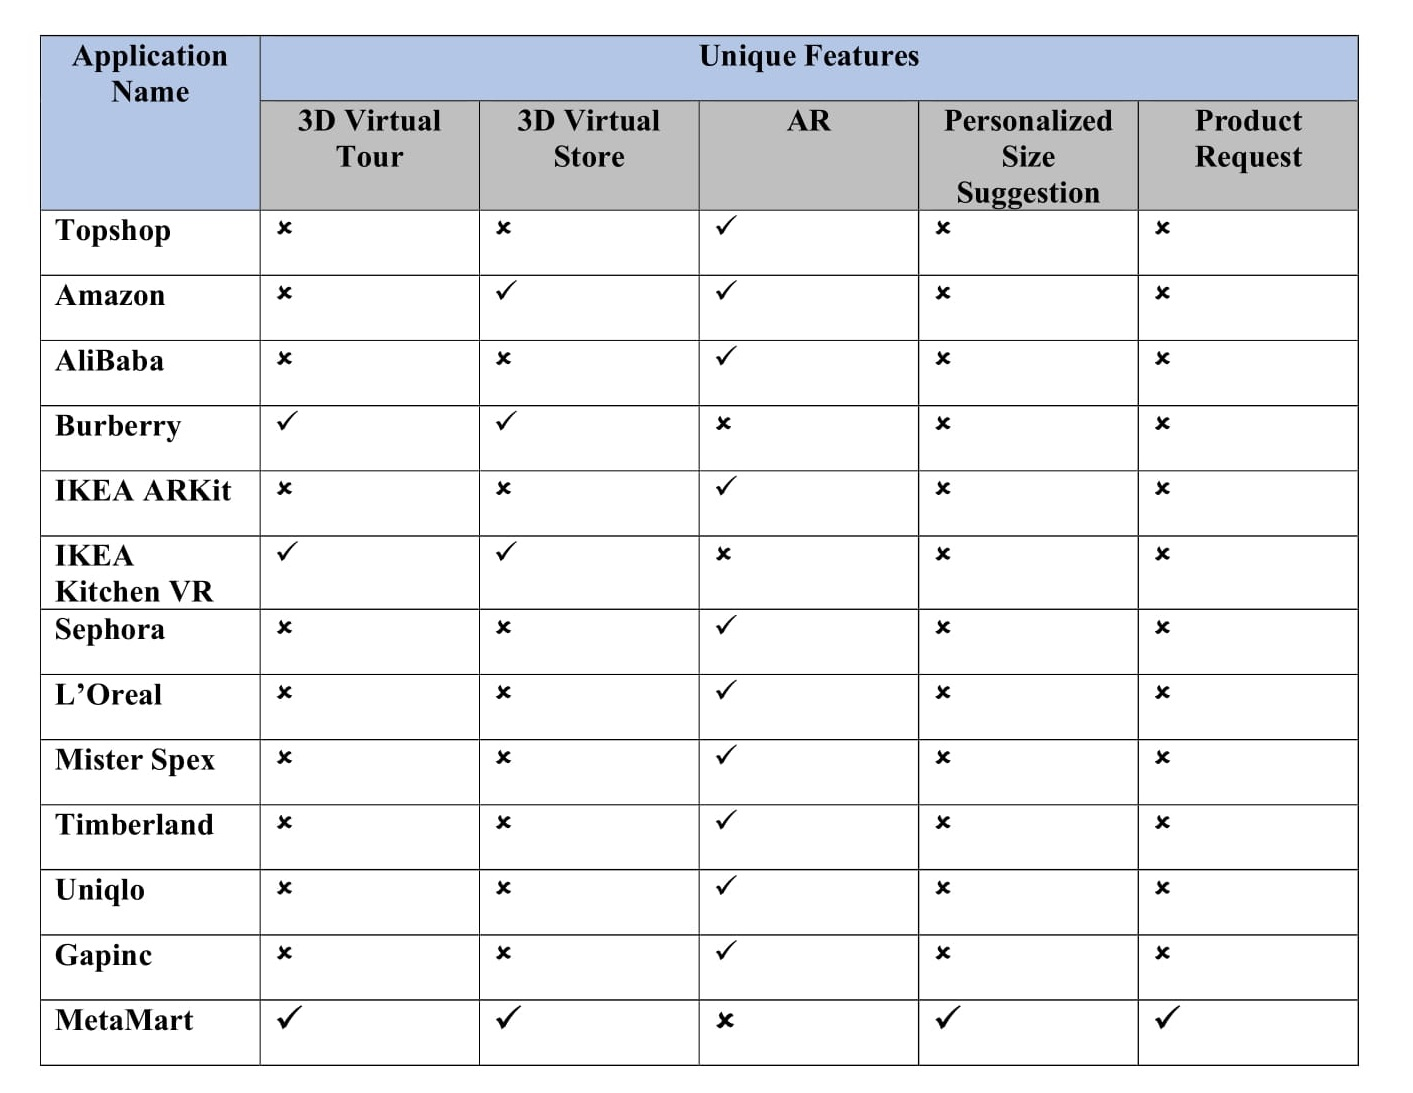
\includegraphics[width=15cm,height=15cm]{Figures/Others/ComparisonTable.jpg}
    \caption{Comparison of existing AR/VR application’s key features}
    \label{fig2:Comparison of existing AR/VR application’s key features}
    \justifying
   This table list some key features and their availability status in existing AR/VR applications. The table shows some features like a 3D virtual tour, 3D virtual store, AR, and personalized size suggestions. Every existing AR/VR application listed in the table has used some of these features not all. But our system would be focusing on all these features.
\end{figure}
